% SIMPLE features + self-consistent exchange-hole functional
% APS two-column (Theory / Numerical implementation / Results) + appendix.
% NOTE: uses the prb substyle (not prl) so that sections are numbered and
% appendices are lettered --- required for the App./Sec. cross-references to
% resolve. Visual style is the same APS two-column reprint. For a strict PRL
% Letter submission, switch to prl and convert numbered refs to named refs
% (or move the appendix to Supplemental Material).
\documentclass[aps,prb,reprint,superscriptaddress,nofootinbib]{revtex4-2}

\usepackage{amsmath,amssymb}
\usepackage{graphicx}
\usepackage{bm}
\usepackage{booktabs}
\usepackage[colorlinks=true,linkcolor=blue,citecolor=blue,urlcolor=blue]{hyperref}

% --- notation macros (kept consistent with the appendix) ---
\newcommand{\rr}{\mathbf{r}}
\newcommand{\uu}{\mathbf{u}}
\newcommand{\rhat}{\hat{\mathbf{u}}}
\newcommand{\kF}{k_{\mathrm{F}}}
\newcommand{\Rad}{R_{\mathrm{ad}}}
\newcommand{\Rc}{R_{c}}
\newcommand{\nin}{n_{\mathrm{in}}}
\newcommand{\nout}{n_{\mathrm{out}}}
\newcommand{\Ylm}{Y^{\mathbb{R}}_{\ell m}}
% placeholder for numbers to be filled from regenerated runs (Phases C/D)
\newcommand{\PH}[1]{\textcolor{red}{\textbf{[#1]}}}
\usepackage{xcolor}

\begin{document}

\title{Scale-invariant multipole local expansion features and a self-consistent
exchange-hole functional}

\author{A.~J.~Medford}
\affiliation{School of Chemical \& Biomolecular Engineering, Georgia Institute of
Technology, Atlanta, Georgia 30332, USA}

\date{\today}

\begin{abstract}
\PH{Abstract handled separately.} We introduce SIMPLE, a complete, orthonormal,
scale-invariant local expansion of the electron density, and use it to build a
self-consistent exchange functional from an explicit model of the exchange hole.
The descriptors reproduce the homogeneous-electron-gas limit by construction,
are exactly rotationally covariant, and remain numerically stable as the density
vanishes. Projecting the Coulomb interaction onto the same orthonormal basis
turns the exchange-energy integral into a closed contraction of monopole
descriptors, yielding a functional that is exact in the homogeneous and
one-electron (Fermi--Amaldi) limits and matches the gradient expansion to second
order. Self-consistent atomic calculations reproduce optimized-effective-potential
exchange potentials and Hartree--Fock energies across the first rows of the
periodic table.
\end{abstract}

\maketitle

% =====================================================================
% Intro placeholder (handled separately) — keep a single orienting line.
% =====================================================================
\PH{Introduction handled separately.}

% =====================================================================
\section{Theory and methods}
% =====================================================================

\subsection{SIMPLE feature definitions}

The SIMPLE features are a \emph{scale-invariant multipole local expansion} of the
electron density --- a local projection onto an orthonormal radial--angular basis,
reconstructed at a density-adaptive radius so the coefficients are dimensionless and
invariant under uniform scaling.

\subsubsection{Projection, orthogonality, and local scale}
\label{sec:features}

Let $\rho_\sigma$ be the spin-$\sigma$ density. About a point $\rr_0$ we project
the local density onto an orthonormal kernel basis on the ball
$B_{\Rc}=\{\rr:|\rr|\le\Rc\}$,
\begin{equation}
\label{eq:projection}
c_{n\ell m}(\rr_0)=\int_{B_{\Rc}} K_{n\ell m}(\rr)\,\rho_\sigma(\rr_0+\rr)\,d^3r .
\end{equation}
The kernel is $K_{n\ell m}(\rr)=R_{n\ell}(r)\,\Ylm(\hat\rr)$, with real spherical
harmonics $\Ylm$ and Dirichlet spherical-Bessel radial
functions $R_{n\ell}(r)=\mathcal N_{n\ell}\,j_\ell(z_{n\ell}r/\Rc)$
($z_{n\ell}$ the positive zeros of $j_\ell$), orthonormal under
$\int_0^{\Rc} r^2 R_{n\ell}R_{n'\ell}\,dr=\delta_{nn'}$; the $c_{n\ell m}$ are
therefore the orthonormal expansion coefficients of the local density inside the
ball. This is the same class of local density expansion used by atomistic descriptors
such as SOAP~\cite{Bartok2013}, ACE~\cite{Drautz2019}, and SNAP~\cite{Thompson2015},
and by convolutional density functionals~\cite{Lei2019,Lei2022,Sahoo2024}.

\paragraph*{Local density scale.}
The local scale is the ball-averaged density and its Fermi wavevector,
$\bar\rho_\sigma(R)=\tfrac{3}{R^3}\int_0^R r^2\rho_{\sigma,00}\,dr$ and
$\bar\kF(R)=(6\pi^2\bar\rho_{\sigma,\mathrm{safe}})^{1/3}$, where $\rho_{\sigma,00}$
is the spherical-average ($\ell=0$) profile of the local density and the smooth
floor $\bar\rho_{\sigma,\mathrm{safe}}=(\bar\rho_\sigma^2+\rho_{\min}^2)^{1/2}$
regularizes vanishing density ($\rho_{\min}$ a small density floor). Using the ball
average rather than the point value is what keeps the features numerically stable as
$\rho\to0$.

\paragraph*{Adaptive radius and the local Wigner--Seitz scale.}
A functional must see the same dimensionless environment regardless of the local
density scale, so the expansion is reconstructed not at the fixed window $\Rc$ but at
a density-adaptive radius $\Rad$ that holds a fixed dimensionless cutoff $\xi^*$,
\begin{equation}
\label{eq:adaptive}
g(\Rad)=\xi^*,\quad g(R)\equiv R\,\bar\kF(R),\quad \Rad\le\Rc\ \text{(clamped)} .
\end{equation}
Because $\Rad\bar\kF=\xi^*$ fixes the enclosed charge
($[\Rad\bar\kF]^3=18\pi^2 M(\Rad)$, with the enclosed monopole moment
$M(R)=\int_0^R r^2\rho_{\sigma,00}\,dr$), $\Rad$ is the local analogue of the
Wigner--Seitz radius: the radius enclosing a fixed amount of charge measured in local
Fermi wavelengths. In practice it is located by a single fixed-stencil ``charge
within a radius'' convolution $M(R)$ and a closed-form inversion of $M(\Rad)=M^*$
(App.~\ref{app:scale}), with no iterative solve. $\Rad$ is a functional of the
density alone and maps exactly to $\Rad/\lambda$ under
$\rho_\sigma(\rr)\mapsto\lambda^3\rho_\sigma(\lambda\rr)$.

\subsubsection{Scale invariance and non-dimensionalization}
\label{sec:scale}

We require features invariant under that uniform scaling. Exact invariance demands
the adaptive cutoff $\Rad\propto\bar\kF^{-1}$ of Eq.~\eqref{eq:adaptive}, which cannot
be a single fixed convolution stencil; SIMPLE keeps a fixed window and reconstructs
the adaptive-window coefficients by a linear map that is exact when the adaptive
radius lies below the cutoff and decays smoothly once $\Rad$ would exceed it.

\paragraph*{Dilation identity.}
A change of variables in Eq.~\eqref{eq:projection} gives the exact covariance of
the coefficients at corresponding cutoffs,
\begin{equation}
\label{eq:dilation}
c_{n\ell m}\bigl[\rho_\lambda;\,R/\lambda\bigr]=\lambda^{3/2}\,
c_{n\ell m}\bigl[\rho;\,R\bigr],
\end{equation}
because the basis depends on $r$ only through the ratio $z_{n\ell}r/R$
(App.~\ref{app:scale}). A uniform scaling thus dilates the radial sampling
wavevectors but loses no information: the descriptors an adaptive cutoff would
produce are recoverable from fixed-window data.

\paragraph*{Mean-split transfer.}
The reconstruction acts on the fluctuation about the window mean --- the constant
maps analytically through the monopole integrals $A_n(R)=\int_{B_R}K_{n00}\,d^3r$,
removing boundary oscillations,
\begin{align}
\label{eq:meansplit}
\tilde c_{n\ell m}&=c_{n\ell m}-\bar\rho_\sigma(\Rc)A_n(\Rc)\,\delta_{\ell0}\delta_{m0},\\
\label{eq:transfer}
c'_{m\ell m'}&=\bar\rho_\sigma(\Rc)A_m(\Rad)\,\delta_{\ell0}\delta_{m'0}\notag\\
&\quad+\sum_{n=0}^{\nin-1}\mathsf M^{(\ell)}_{mn}(\Rad)\,\tilde c_{n\ell m'} ,
\end{align}
with transfer matrices $\mathsf M^{(\ell)}_{mn}(\Rad)=\int_0^{\Rad}r^2
R^{(\Rad)}_{m\ell}R^{(\Rc)}_{n\ell}\,dr$. For a uniform density $\tilde c\equiv0$,
so the HEG limit is exact at any truncation. Surplus inner channels
($\nin>\nout$) supply the radial resolution the transfer consumes
($\nin\lesssim\Rc/2h$ on a grid of spacing $h$).

\paragraph*{Closed form.}
With $a=z_{m\ell}/\Rad$ and $b=z_{n\ell}/\Rc$, the Sturm--Liouville cross-product
identity evaluates the transfer matrices analytically, with no quadrature or
tabulation,
\begin{equation}
\label{eq:transfer-closed}
\begin{aligned}
&\int_0^{R} r^2 j_\ell(ar)j_\ell(br)\,dr\\
&\qquad=\frac{R^2\bigl[a\,j_\ell'(aR)j_\ell(bR)-b\,j_\ell(aR)j_\ell'(bR)\bigr]}{b^2-a^2},
\end{aligned}
\end{equation}
which at $R=\Rad$ simplifies further since $j_\ell(a\Rad)=j_\ell(z_{m\ell})=0$
(App.~\ref{app:scale}).

\paragraph*{Non-dimensionalization.}
\label{sec:nondim}
The SIMPLE features normalize the transferred coefficients by the local amplitude
scale at the adaptive radius,
\begin{equation}
\label{eq:dnlm}
\varrho_{n\ell m}(\rr_0)=\frac{c'_{n\ell m}(\rr_0)}
{A_0(\Rad)\,\bar\rho_{\sigma,\mathrm{safe}}(\Rad)} ,
\end{equation}
which is dimensionless for every $\ell$ and, by Eqs.~\eqref{eq:dilation} and
\eqref{eq:transfer}, exactly invariant under uniform scaling in the continuum
(App.~\ref{app:nondim}). The ball average gives a smooth $\rho\to0$ limit,
$\varrho_{n\ell m}=\mathcal O(\epsilon)$ and power spectrum $\sim\mathcal O(\epsilon^2)$
as $\rho\to\epsilon\rho$, with no overflow. After non-dimensionalization the
homogeneous-gas limit is the fixed analytic vector
$\varrho^{\mathrm{HEG}}_{n00}=(-1)^n/(n+1)$, $\varrho_{n\ell m}=0\,(\ell>0)$: a uniform
density carries only this monopole signature, and any departure from it measures
inhomogeneity. The local scale $\bar\kF$ is retained as an explicit feature --- the
physically correct factorization, since exchange obeys
$E_x[\rho_\lambda]=\lambda E_x[\rho]$ while correlation requires the scale.

The SIMPLE features $\varrho_{n\ell m}$ are thus a scale-free, orthonormal expansion
of the density about a point --- dimensionless, smoothly behaved in vacuum, and
systematically improvable as $\Rc$ and the channel resolution increase.

\subsection{Construction of SIMPLE invariants}
\label{sec:invariants}

Under a rotation $\mathcal R$ the features transform as rank-$\ell$ spherical
tensors, $\varrho_{n\ell m}\mapsto\sum_{m'}D^{(\ell)}_{mm'}(\mathcal R)\,\varrho_{n\ell m'}$
(App.~\ref{app:nondim}): they are rotationally \emph{covariant}, whereas a density
functional needs inputs that are rotationally \emph{invariant}. We construct
invariants in three ways --- the dimensionless reduced gradient and Laplacian, the
power spectrum and bispectrum that form a complete basis, and targeted projections of
specific physical operators.

\subsubsection{Dimensionless gradient and Laplacian}
\label{sec:gea}

The dimensionless inhomogeneity measures used by semilocal functionals --- the reduced
gradient $s=|\nabla\rho|/(2\kF\rho)$ and reduced Laplacian $q=\nabla^2\rho/(4\kF^2\rho)$
(with $\kF=(3\pi^2\rho)^{1/3}$) --- are recovered directly from the SIMPLE features,
with no fit or empirical decoder. Since $\nabla\rho$ is a vector (rank $1$) and
$\nabla^2\rho$ a scalar (rank $0$), they are spectral contractions of the $\ell=1$ and
$\ell=0$ channels,
\begin{equation}
\label{eq:sq}
s=c_s\sqrt{\sum_{m}\Big(\sum_n g^{(1)}_n\,\varrho_{n1m}\Big)^2},\qquad
q=c_q\sum_n g^{(0)}_n\,\varrho_{n00},
\end{equation}
with fixed parameter-free spectral weights --- $g^{(1)}_n\propto R'_{n1}(0)$ (the
slope at the origin) and $g^{(0)}_n\propto k_n^2 R_{n0}(0)$ (the Bessel eigenvalue,
$k_n=z_{n0}/\Rc$) --- and constants $c_s,c_q$ (App.~\ref{app:gea}). The
non-dimensionalization already supplies the $1/(2\kF\rho)$ and $1/(4\kF^2\rho)$
factors, so $s$ is simply the $\ell=1$ power of the spectrally-weighted features and
inherits their rotational and scale invariance.

The two ingredients differ sharply in practice. The reduced gradient is well-behaved,
agreeing with direct finite differences to $\sim1\%$ within the basis resolution
(Sec.~\ref{sec:results-cartesian}). The reduced Laplacian is recoverable by the same
construction but \emph{not numerically usable}: like a standard finite-difference
Laplacian, the $\ell=0$ eigenvalue sum weighted by $k_n^2$ amplifies high-wavevector
noise, and its relative reconstruction error reaches tens to hundreds of percent in
dense environments (Sec.~\ref{sec:results-cartesian}, App.~\ref{app:gea}). The reduced
gradient is therefore a reliable ingredient and the Laplacian is not.

\subsubsection{Power spectrum, bispectrum, and operator projections}
\label{sec:operators}

Because the transfer acts on the radial index $n$ while rotations act on the magnetic
index $m$, the two commute, so any contraction of the $\varrho_{n\ell m}$ to total
angular momentum zero is a rotational invariant (App.~\ref{app:nondim}). Two routes
are useful. Generic invariants form a \emph{complete basis} for rotationally invariant
multilinear functionals of the density --- the power spectrum
$\tilde P_{n\ell}=\sum_m \varrho_{n\ell m}^2$, the bispectrum, and higher
Clebsch--Gordan trees --- systematically improvable as $\Rc$ and the resolution
increase. This route is especially favorable for machine-learned functionals: rather
than a fixed, hand-chosen descriptor set, the model is handed a complete, orthonormal,
systematically convergent projection of the local environment, so its accuracy can be
improved in a controlled way simply by extending the basis. Alternatively one can
\emph{target a specific operator} whose symmetry is known and project it directly onto
the features.

The decisive targeted example is the Coulomb operator $1/u$. Orthonormality converts
any rotation-invariant $\nu$-point kernel into a finite contraction
$\sum T^{(\nu)}_{\{n_i\ell_i m_i\}}\prod_i \varrho_{n_i\ell_i m_i}$ with constant
projected-kernel coefficients (App.~\ref{app:operators}); for $1/u$ only the monopole
($\ell=0$) average of the density survives the isotropic angular integral,
$\bar\rho(r_0,u)=\sum_n C_n(r_0)R_n(u)$ with
$C_n=A_0(\Rad)\,\bar\rho_{\sigma,\mathrm{safe}}(\Rad)\,\varrho_{n00}$ [the dimensional
form of Eq.~\eqref{eq:dnlm}], and the operator is the radial Coulomb contraction
\begin{equation}
\label{eq:coulomb}
\begin{aligned}
\int_{B_{\Rc}}\!\frac{\rho(r_0+\uu)}{u}\,d^3u
&=4\pi\!\int_0^{\Rc}\!\bar\rho(r_0,u)\,u\,du\\
&=\sum_n w_n\,C_n(r_0),
\end{aligned}
\end{equation}
with weights $w_n=4\pi\int_0^{\Rc}R_n(u)\,u\,du$. The $1/u$ weight reduces the volume
measure $u^2du$ to $u\,du$: the projection keeps the long-range $1/r$ dependence that
semilocal functionals miss --- it is \emph{not} merely the average density. Contracted
with the local density itself, Eq.~\eqref{eq:coulomb} is the Hartree energy of the
environment enclosed within $\Rc$, so the Coulomb projection converts the density
directly into an approximate local energy scale (used in Sec.~\ref{sec:results-scale}
to calibrate $\Rc$ and $\nout$). More generally, projecting other physical operators
onto the features in the same way supplies the building blocks for physics-based
functionals.

\subsection{Exchange-hole functional}
\label{sec:hole}

\emph{(This subsection records the current exchange-hole construction; the functional
itself is under active development, and the self-consistent benchmarks of
Sec.~\ref{sec:results-hole} are preliminary. The feature and invariant constructions
above are finalized.)}

Exchange is exactly a hole integral,
\begin{equation}
\label{eq:exact-hole}
E_x[\rho]=\tfrac12\int d^3r_0\,\rho(r_0)\!\int d^3u\,\frac{n_x(r_0,\uu)}{u} ,
\end{equation}
where $\uu$ is the displacement between the two electrons and $u=|\uu|$: around each
electron at $r_0$ sits an exchange hole $n_x\le0$ that removes exactly one electron
from the surroundings ($\int n_x\,d^3u=-1$), and $E_x$ is the electrostatic
attraction between the electron and that hole. We model the hole as the neighboring
density itself, damped by one universal screening envelope $S$,
\begin{equation}
\label{eq:ansatz}
n_x(r_0,\uu)=-W(r_0)\,\rho(r_0+\uu)\,S\!\big(\zeta(r_0)\,u\big),
\end{equation}
where $S$ falls from $S(0)=1$ to zero beyond a screening length $1/\zeta$. The two
local scalars --- the scale $\zeta$ and weight $W$ --- are fixed by exact sum rules
(the hole holds one electron and equals half the density on top of $r_0$;
App.~\ref{app:hole}). The entire functional then reduces to a single choice: the
shape $S$.

\paragraph*{The enhancement factor as an integral over $S\rho$.}
Inserting Eq.~\eqref{eq:ansatz} into Eq.~\eqref{eq:exact-hole}, the exchange energy
per electron is the self-repulsion of the enclosed density divided by the charge it
holds,
\begin{equation}
\label{eq:eps-x}
\varepsilon_x(r_0)=-\tfrac12\,\frac{\Phi_S(\zeta^*)}{Q_S(\zeta^*)},
\end{equation}
where, with $\bar\rho(u)$ the spherical average of $\rho(r_0+\uu)$ that the $1/u$
weight selects, $Q_S(\zeta)=4\pi\!\int_0^{\Rad}S(\zeta u)\bar\rho(u)u^2du$ is the
charge enclosed and $\Phi_S(\zeta)=4\pi\!\int_0^{\Rad}S(\zeta u)\bar\rho(u)u\,du$ its
self-repulsion (the $1/u$ turning $u^2du$ into $u\,du$), and $\zeta^*$ is fixed by
$Q_S=2$. The dimensionless enhancement factor
$F_x=\varepsilon_x/\varepsilon_x^{\mathrm{unif}}$, with
$\varepsilon_x^{\mathrm{unif}}=-\tfrac34(3/\pi)^{1/3}\rho^{1/3}$, is then explicitly
an integral of the shape $S$ against the density,
\begin{equation}
\label{eq:Fx-S}
F_x[S]=-\frac{1}{2\,\varepsilon_x^{\mathrm{unif}}}\,
\frac{\displaystyle\int_0^{\Rad} S(\zeta^* u)\,\bar\rho(u)\,u\,du}
     {\displaystyle\int_0^{\Rad} S(\zeta^* u)\,\bar\rho(u)\,u^2\,du}.
\end{equation}
This says how much the local environment raises or lowers exchange relative to LDA.
$F_x$ is manifestly a functional of the shape $S$; being a ratio of energies it is
dimensionless, and because $\zeta^*\propto\rho^{1/3}$ the density scale cancels
between numerator and denominator, so $F_x$ depends only on the \emph{shapes} of $S$
and of the local density --- it is automatically scale-invariant. Designing the
functional means shaping $S$ to meet the exact constraints
\begin{itemize}\setlength{\itemsep}{0pt}
\item[(C1)] negativity and the normalization sum rule;
\item[(C2)] spin-scaling;
\item[(C3)] uniform-density scaling $E_x[\gamma^3\rho(\gamma r)]=\gamma E_x[\rho]$;
\item[(C4)] the homogeneous-gas (LDA) limit $F_x\to1$;
\item[(C5)] the Fermi--Amaldi one-electron limit;
\item[(C6)] the second-order gradient expansion $F_x\to1+\tfrac{10}{81}s^2$;
\item[(C7)] the Lieb--Oxford bound $F_x\le1.804$.
\end{itemize}

\paragraph*{Projecting $S$ onto the SIMPLE features.}
The integrals in Eq.~\eqref{eq:eps-x} collapse to dot products in the SIMPLE basis.
The $1/u$ weight keeps only the spherical ($\ell=0$) part of the surrounding
density, whose basis coefficients are the monopole features
$\mathbf C=(C_0,C_1,\dots)$, $C_n=A_0(\Rad)\bar\rho_{\sigma,\mathrm{safe}}(\Rad)\,\varrho_{n00}$;
and the shape $S$ projects onto the same basis as fixed envelope tables
$\bm\alpha,\bm\beta$ (entries $\alpha_n(\zeta)=\int_0^\infty S(\zeta u)R_n(u)u^2du$,
$\beta_n(\zeta)=\int_0^\infty S(\zeta u)R_n(u)u\,du$). The two pieces are then simply
\begin{equation}
\label{eq:QPhi}
Q_S(\zeta)=\bm\alpha(\zeta)\!\cdot\!\mathbf C,\qquad
\Phi_S(\zeta)=\bm\beta(\zeta)\!\cdot\!\mathbf C,
\end{equation}
so $F_x$ is a closed function of the SIMPLE features (the tables are evaluated in
App.~\ref{app:hole}). Forming $\mathbf C$ on the adaptive radius --- i.e.\ from the
scale-invariant features $\varrho_{n00}$ [Eqs.~\eqref{eq:dnlm},~\eqref{eq:transfer}]
rather than the fixed window --- makes uniform scaling (C3) exact as $R_c\to\infty$
and close for finite $R_c$ within the data window (Fig.~\ref{fig:hole-scale}).

\paragraph*{From the SIMPLE features to the gradient expansion.}
It remains to choose $S$. Fixing it to the homogeneous-gas hole shape
$S(x)=[3j_1(x)/x]^2=[j_0(x)+j_2(x)]^2$ makes $F_x=1$ at uniform density (LDA, C4) and,
where the hole cannot enclose two electrons, reduces $\varepsilon_x$ to the exact
one-electron self-interaction correction (Fermi--Amaldi, C5). For a varying density
the small-gradient behaviour of $F_x$ must match the exact gradient expansion. The
spherical average is blind to $\nabla\rho$, so the undeformed shape misses the
gradient term; we restore it by deforming the envelope,
$S(x;\chi)=[g_0(x)+\chi\,\phi(x)]^2$ ($g_0=3j_1/x$, mode $\phi=j_1$), and tying the
single amplitude $\chi$ to the SIMPLE reduced gradient $s$ (from the $\ell=1$
features, Eq.~\eqref{eq:sq}). To linear order the deformation simply scales the
enhancement, $F_x=1+R\,\chi$, with $R$ a fixed homogeneous-gas constant (one number,
because the hole is scale-free); choosing
\begin{equation}
\label{eq:amp}
\chi=\frac{1}{R}\,\tfrac{10}{81}\,s^2
\end{equation}
therefore reproduces the exact second-order gradient expansion,
\begin{equation}
\label{eq:fx}
F_x\;\xrightarrow[\,s\to0\,]{}\;1+\tfrac{10}{81}\,s^2 ,
\end{equation}
with no fitted numbers (App.~\ref{app:hole} derives $R$ and the deformation tables).
Because $\phi(0)=0$ the deformation never changes the on-top value, so LDA and
Fermi--Amaldi survive for any $\chi$. Finally, the gradient expansion grows without
bound at large $s$, so $\chi$ is smoothly capped,
$\chi\to\chi_{\max}\tanh(\chi/\chi_{\max})$, with the ceiling $\chi_{\max}$ set by the
Lieb--Oxford bound $F_x\le1.804$ (C7)~\cite{Lieb_1981,Perdew_1996} --- a
parameter-free, PBE-style saturation.

\begin{figure}[tbp]
\centering
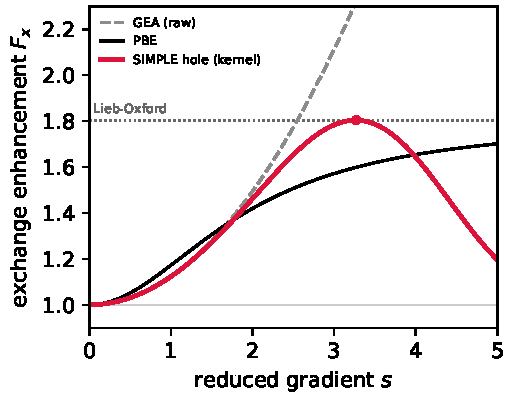
\includegraphics[width=\columnwidth]{figures/fx_enhancement.pdf}
\caption{Exchange enhancement factor of the scale-free SIMPLE hole. The analytic
second-order gradient expansion [Eq.~\eqref{eq:fx}] sets the small-$s$ slope to the
exact $\mu=10/81$; the deformation amplitude is then smoothly saturated, with the
ceiling $\chi_{\max}$ fixed by the local Lieb--Oxford bound $F_x\le1.804$ (dotted).
The realized GEA2 enhancement (solid, the re-summed hole
$F_x=\varepsilon_x/\varepsilon_x^{\mathrm{LDA}}$ on the homogeneous gas at the
adaptive window) tracks the exact slope at small $s$, then saturates below the LO
bound where the raw pointwise GEA (grey dashed) diverges --- a
PBE-like~\cite{Perdew_1996} (black) saturation arising here from the Lieb--Oxford
ceiling rather than a fitted parameter. The on-top value $S(0)=1$ is preserved for
any amplitude, so the Fermi--Amaldi limit is untouched.}
\label{fig:fx}
\end{figure}

\begin{figure}[tbp]
\centering
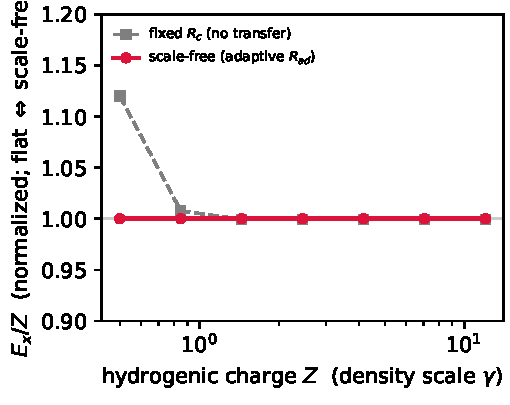
\includegraphics[width=\columnwidth]{figures/scale_invariance_hole.pdf}
\caption{Uniform-scaling (scale invariance) of the hole on atoms. For the hydrogenic
density $\rho_Z=(Z^3/\pi)e^{-2Zr}$ the map $Z\!\to\!\gamma Z$ is the uniform scaling
$\rho\!\to\!\gamma^3\rho(\gamma r)$, so the exact constraint
$E_x[\rho_\gamma]=\gamma E_x[\rho]$ requires $E_x/Z$ to be $Z$-independent. The
scale-free hole (adaptive radius $\Rad$, reached by the transfer) is flat to machine
precision; the fixed-$R_c$ hole (no transfer) drifts once the density is diffuse
enough to overflow the window. $R_c$ remains the explicit data window, and scale
invariance holds within it.}
\label{fig:hole-scale}
\end{figure} The hole is spherically symmetric and so uses no multipoles beyond
those in Eqs.~\eqref{eq:eps-x}--\eqref{eq:amp}; carrying explicit $\ell\ge1$ hole
multipoles is the natural route to a richer functional (App.~\ref{app:hole}).

\paragraph*{Spin.}
Everything above is stated for the general spin-resolved hole. The exchange energy
decomposes exactly as
$E_x[\rho_\uparrow,\rho_\downarrow]=\tfrac12(E_x[2\rho_\uparrow]+E_x[2\rho_\downarrow])$,
so the spin-paired functional follows from the total-density expressions with the
on-top count of $2$, and the open-shell case is obtained by applying the
spin-scaling relation to each channel (App.~\ref{app:spin}).

Constraints (C1)--(C7) are thus all satisfied by construction rather than by
fitting. Those requiring the kinetic-energy density --- the tight single-orbital
Lieb--Oxford bound $F_x(s,\alpha{=}0)\le1.174$ and one-electron self-correlation
freedom --- lie outside this orbital-free, exchange-only construction.

\subsection{Direct-expansion hole and gradient-corrected functional}
\label{sec:hole-expansion}

\emph{(This subsection records a second, more flexible hole construction built on the
same features and a gradient correction with an iso-orbital gate; it is under active
development and the self-consistent benchmarks reported here are preliminary.)}

The single-envelope model [Eq.~\eqref{eq:ansatz}] fixes the hole to one universal
shape $S$ scaled by $\zeta$. A more flexible construction expands the
spherically-averaged hole monopole \emph{directly} in the scale-free SIMPLE radial
basis,
\begin{equation}
\label{eq:hole-direct}
\bar n_x(r_0,u)=\sum_n \tilde\varrho_{n}(r_0)\,R_{n0}(u),
\end{equation}
so the hole is a vector of coefficients $\{\tilde\varrho_n\}$ rather than a single
scale. Because the $1/u$ weight keeps only the monopole, the energy per electron
[Eq.~\eqref{eq:exact-hole}] is a dot product,
\begin{equation}
\label{eq:eps-direct}
\varepsilon_x(r_0)=2\pi\sum_n \tilde\varrho_n(r_0)\,b_n,\qquad
b_n=\int_0^{\Rc}\!R_{n0}(u)\,u\,du ,
\end{equation}
and the exact constraints become linear in $\{\tilde\varrho_n\}$: the normalization
sum rule $4\pi\sum_n\tilde\varrho_n a_n=-1$ (with $a_n=\int_0^{\Rc}R_{n0}u^2du$ the
enclosed charge) and the on-top value. The coefficients are produced by a
parameter-free map of the local monopole features that interpolates between the
homogeneous-gas hole (LDA limit, C4) and the negative of the local density
(Fermi--Amaldi one-electron limit, C5), formed on the same adaptive-radius frame
[$\Rad=\min(\xi^*/\kF,\Rc)$, Eq.~\eqref{eq:transfer}] so uniform scaling (C3) holds
within the window. With the on-top scale fixed by the enclosed-charge sum rule
($Q_S{=}2$), hydrogen is reproduced to $\sim2$~mHa (a near-exact self-interaction
correction), spin-paired He to $\sim2$~mHa, and Be within $\sim2\%$.

\paragraph*{Gradient correction with an iso-orbital gate.}
The monopole hole is blind to $\nabla\rho$, so as before a gradient correction must
be added. Here it is built from \emph{two} gated terms acting on the LDA enhancement,
\begin{equation}
\label{eq:F-twoterm}
\varepsilon_x=\varepsilon_x^{0}\,F,\qquad
F=1+s^2\big(m_g\,g_{\mathrm{HEG}}+m_h\,g_{\mathrm{H1s}}\big),
\end{equation}
where $\varepsilon_x^{0}$ is the gradient-free direct-expansion energy and $s$ is the
SIMPLE reduced gradient [Eq.~\eqref{eq:sq}]. The gates are pure \emph{point-wise}
squared distances of the local scale-free features from two fixed reference
signatures,
$g_{\mathrm{HEG}}=e^{-\alpha_{\mathrm{HEG}}D_{\mathrm{HEG}}}$ and
$g_{\mathrm{H1s}}=1-e^{-\alpha_{\mathrm{H1s}}D_{\mathrm{H1s}}}$, with
$D_{\mathrm{HEG}}$ the distance from the uniform-gas signature and $D_{\mathrm{H1s}}$
the distance from a hydrogenic-$1s$ signature (each a single feature vector, so the
gate carries over to three dimensions unchanged). Both terms carry $s^2$, so the
homogeneous limit ($s\to0$) is untouched (C4); $g_{\mathrm{H1s}}$ vanishes on the
single-orbital manifold, so the one-electron limit (C5) survives. The two terms have
opposite sign and are tied so they \emph{cancel} for a spin-paired two-electron atom,
which preserves the Fermi--Amaldi limit there and fixes the ratio $m_h/m_g$; the
overall magnitude $m_g$ is then the single calibrated degree of freedom, set on the
heavier closed-shell atoms.

\paragraph*{Tail instability and damping.}
The raw factor in Eq.~\eqref{eq:F-twoterm} is not bounded below. In the low-density
tail the reduced gradient saturates while the HEG gate stays finite, so with the
calibrated (large, negative) $m_g$ the factor passes through zero and turns negative;
$F<0$ flips the sign of $\varepsilon_x$ (a spurious \emph{positive} exchange-energy
density), which makes the self-consistent exchange potential diverge and the SCF fail
to converge --- a structural failure of the bare form, present even at a quarter of
the calibrated magnitude. We damp it with a soft floor in the spirit of the LB94
asymptotic correction~\cite{vanLeeuwen_1994},
\begin{equation}
\label{eq:F-floor}
F=F_0+\tfrac1k\ln\!\Big(1+e^{\,k\,(1+e-F_0)}\Big),\qquad
e=s^2\big(m_g g_{\mathrm{HEG}}+m_h g_{\mathrm{H1s}}\big),
\end{equation}
which is the identity in the bulk (where $1+e$ is well above $F_0$) and lifts $F$
smoothly to a small positive floor $F_0$ only in the tail, keeping
$\varepsilon_x<0$ and the potential finite. With the floor and a potential that
freezes the enhancement factor when it is differentiated, the functional converges
self-consistently for the closed-shell atoms tested. Two caveats are worth recording.
First, the floor removes a genuinely \emph{unphysical} negative-$F$ contribution that
had artificially lowered the non-self-consistent tail energy, so the floored,
physical functional is less accurate than that uncorrected estimate suggested.
Second, the two-term cancellation that pins the Fermi--Amaldi limit is imposed on a
fixed density and drifts by a few mHa once the density relaxes self-consistently.
Across He, Be, Na, and Mg (pseudopotential, valence only) the self-consistent
exchange energies reach a mean absolute error of $\sim\!30$~mHa against the exact
(optimized-effective-potential) reference --- roughly three times closer than PBE
exchange and five times closer than the gradient-free hole --- with a residual
over-binding of $40$--$60$~mHa on Na and Be that remains the target of further work.
The all-electron core is excluded deliberately: there the adaptive window collapses
($\Rad\!\to\!0$ at the nuclear cusp) and the fixed-$\Rc$ transfer no longer resolves
the hole, a separate breakdown outside the pseudopotential regime in which the
functional is intended to operate.

\subsection{Numerical implementation}
\label{sec:impl}

\paragraph*{Convolutions and spectral operators.}
Every descriptor is a fixed-stencil convolution of the density. The reduced-gradient
ingredient of Sec.~\ref{sec:gea} is evaluated by a parameter-free spectral operator:
the $\ell=1$ slope-at-origin sum $\rho'(r_0)=\sum_n a^{(1)}_n R'_{n1}(0)$ (with a
constant-annihilation correction enforcing the uniform-density limit; $a^{(1)}_n$ the
$\ell=1$ channel coefficients), a fixed linear stencil on the gridded density. So
formed, $|\nabla\rho|$ is recovered to $\sim1\%$ in the core/valence of smooth
(pseudopotential) atoms (App.~\ref{app:gea}).

\paragraph*{Self-consistent potential.}
The exchange potential is the explicit variational derivative
$v_x=\delta E_x/\delta\rho$, which for convolutional descriptors is itself a
convolution over the kernel [Eq.~\eqref{eq:adjoint}], following
Ref.~\cite{Sahoo2024}; in the radial implementation it is the transpose of the
forward stencils. The on-top scale $\zeta(r_0)$ is obtained without an inner
self-consistency loop: $Q_S(\zeta)=\bm\alpha(\zeta)\cdot\mathbf C$ is monotonic in
$\zeta$, so inverting $Q_S=2$ pointwise on the precomputed envelope table is the
same fixed-stencil enclosed-charge solve used for the adaptive radius $\Rad$
(Sec.~\ref{sec:features}), vectorized over all grid points (App.~\ref{app:hole-numerics}).
The asymptotic $-1/r$ exchange tail is recovered by an energy-neutral gauge fix plus a
low-density damping (App.~\ref{app:hole-numerics}). The $\ell=1$ gradient deformation
[Eq.~\eqref{eq:amp}] enters the potential through its own adjoint, which --- growing
only as $k_n^1$ --- is well-conditioned, so the second-order functional is
self-consistent and stable without any auxiliary loop (App.~\ref{app:hole-numerics}).

\paragraph*{Code and tests.}
The functional is implemented in the \texttt{atom-dft} finite-element radial
Kohn--Sham code~\cite{Kohn_1965,Hohenberg_1964} (all-electron and
pseudopotential). Descriptor tests use two independent grids --- a radial
finite-element grid and a 3D Cartesian finite-difference grid carrying
pseudo-H$_2$/N$_2$ densities. The test harness was driven in part by an agentic AI
assistant, with every reported result reproduced by the shipped scripts.

% =====================================================================
\section{Results}
% =====================================================================

\subsection{Numerical validation of SIMPLE feature properties}
\label{sec:results-features}

The features are validated on two independent grids --- a radial finite-element grid
and genuine 3D Cartesian lattices carrying superposition densities (pseudo-H$_2$,
pseudo-N$_2$, pseudo-H$_2$O, and FCC bulk Al and Pt) --- at realistic settings, to
establish the practical limits of each feature family. Unless noted, $\ell_{\max}=3$.

\subsubsection{Orthogonality and limiting behavior}
\label{sec:results-ortho}

The features reproduce the analytic HEG values
$\varrho^{\mathrm{HEG}}_{n00}=(-1)^n/(n+1)$, $\varrho_{n\ell m}=0\,(\ell>0)$ to
$\sim2\times10^{-11}$ in the continuum and to $<4\times10^{-3}$ on the $h=0.2$~bohr
grid (SI Fig.~\ref{fig:heg}), degrading only as the channel count approaches the
Nyquist bound $\nin\lesssim\Rc/2h$. As the density is scaled toward vacuum the
coefficient norm and power spectrum decay as
$\mathcal O(\epsilon)/\mathcal O(\epsilon^2)$ (fitted slope $2.000$; SI
Fig.~\ref{fig:vacuum}), so the features vanish smoothly rather than diverging --- the
property that lets them be evaluated in the tail regions of real atoms.

\subsubsection{Radial scale and scale invariance}
\label{sec:results-scale}

\emph{Scale invariance.} Under $\rho\mapsto\lambda^3\rho(\lambda\rr)$ the relative
deviation at $\lambda=2$ is $0.35$--$1.7\%$ in the continuum, versus $170\%$ for the
untransformed fixed-window features (Fig.~\ref{fig:scale}); the residual is set by
the inner-channel resolution bound and the low-density window clamp of
Sec.~\ref{sec:scale}.

\emph{Choosing $\Rc$ and $\nout$ by an energy scale.} The window cutoff and channel
count are fixed not by inspection but by a target energy accuracy. Evaluating the
Hartree self-energy of the hydrogen $1s$ density through the SIMPLE Coulomb projection
[Eq.~\eqref{eq:coulomb}] against the exact $5/16$~Ha (Fig.~\ref{fig:params}), the
window (Coulomb-tail) floor reaches the milli-Hartree scale only at $\Rc\gtrsim6$~bohr
($-1.7$~mHa at $\Rc=5$, $-0.4$~mHa at $\Rc=6$), while the radial-basis error falls
below $1$~mHa by $\nout\approx8$ and reaches that floor by $\nout=10$ ($-0.5$~mHa).
On a real Cartesian grid this tolerance is registration-robust for
$h\lesssim0.2$--$0.25$~bohr and reaches the $\pm1$~mHa edge only at $h=0.3$
(Fig.~\ref{fig:params}c). We therefore adopt $\Rc=6$~bohr and $\nout=10$ throughout.

\emph{Cost.} With $\nin=\Rc/h$ grid-resolved inner channels the scale transform is
invariant up to a dilation $\Lambda_{\max}\simeq\nin/\nout$, and the feature set costs
$N_{\mathrm{conv}}=\nin(\ell_{\max}+1)^2$ convolutions. The cost is set by the target
scale range, not the grid: fixing $\nin=\nout\Lambda$ holds $N_{\mathrm{conv}}$ fixed
across $h$ (finer grids only sharpen the same channels; App.~\ref{app:params}). At
$\nin=20$ (covering $\Lambda=2$ for $\nout=10$) the full feature set is
$N_{\mathrm{conv}}=320,180,80$ convolutions for $\ell_{\max}=3,2,1$ on any grid
$h\le0.3$~bohr.

\begin{figure}[tb]
\centering
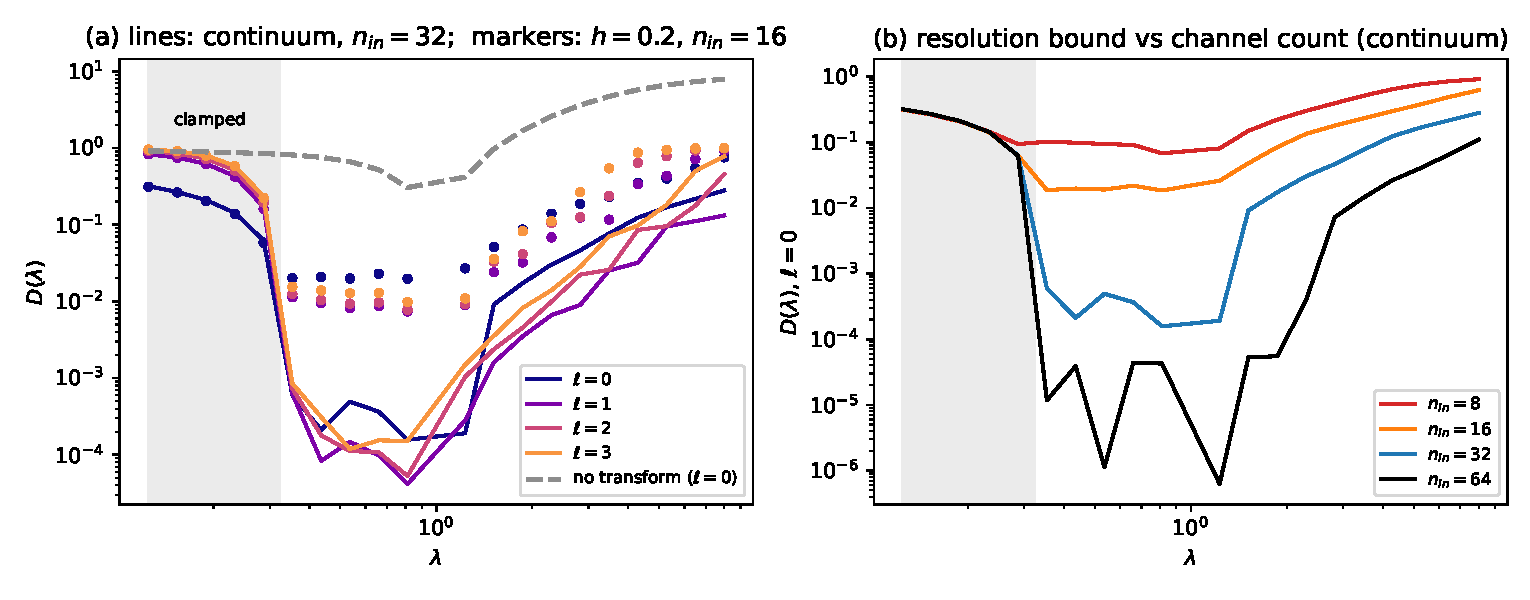
\includegraphics[width=\columnwidth]{figures/simple_scale.pdf}
\caption{Scale invariance of the SIMPLE features under uniform scaling
$\rho\mapsto\lambda^3\rho(\lambda\rr)$ (Sec.~\ref{sec:scale}) and its two breakdown
mechanisms; $D(\lambda)=\lVert \varrho(\lambda)-\varrho(1)\rVert/\lVert \varrho(1)\rVert$
is the relative deviation of the feature vector from its unscaled ($\lambda=1$) value.
\textbf{(a)} $D(\lambda)$ for the channels $\ell=0$--$3$: solid lines are the
continuum quadrature ($\nin=32$ inner channels) and markers the $h=0.2$~bohr grid
with the grid-matched count ($\nin=16$). The gray dashed line is the untransformed
fixed-window baseline ($\ell=0$, no scale transform), which deviates at the
$\mathcal O(1)$ ($\sim$170\%) level. In the shaded region
($\lambda<\lambda_{\mathrm{clamp}}\approx0.32$) the adaptive radius is clamped at
the window ($\Rad=\Rc$) and the features revert continuously to fixed-window
behavior. \textbf{(b)} The resolution mechanism isolated ($\ell=0$, continuum):
$D(\lambda)$ for increasing inner-channel counts $\nin\in\{8,16,32,64\}$; the
deviation falls systematically with $\nin$, and the usable dilation range grows as
$k^*\lambda\lesssim\nin\pi/\Rc$ (on a grid $\nin\lesssim\Rc/2h$).}
\label{fig:scale}
\end{figure}

\begin{figure}[tb]
\centering
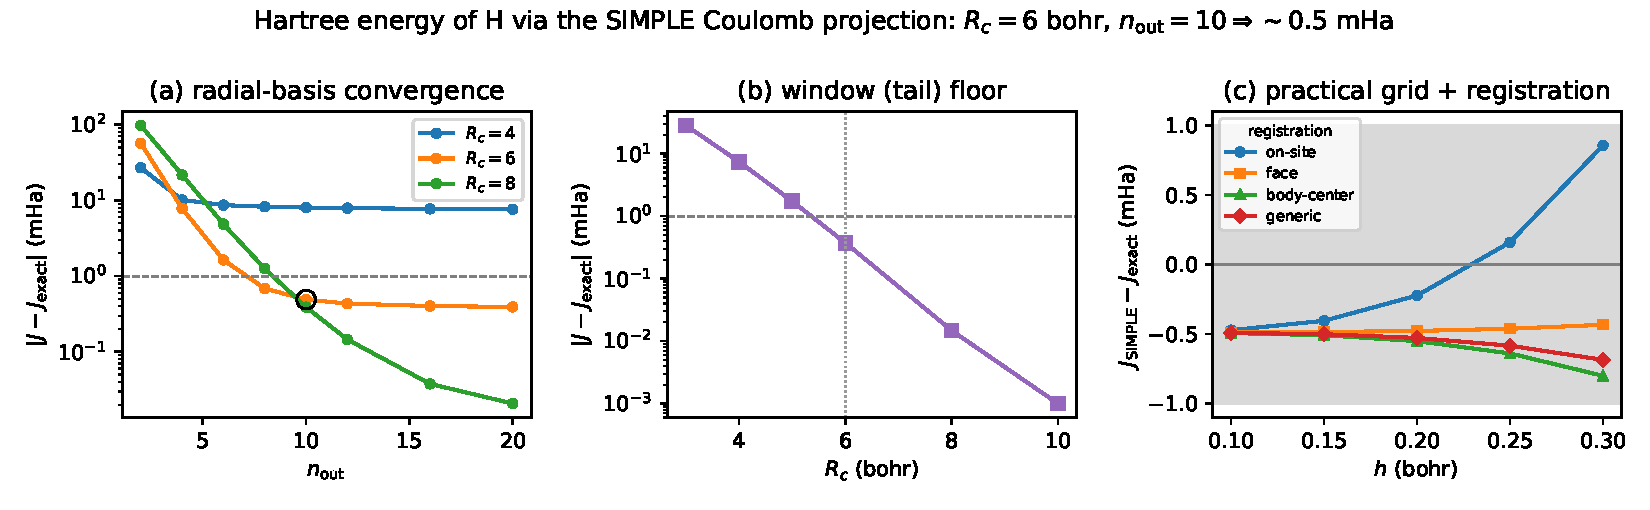
\includegraphics[width=\columnwidth]{figures/params_main.pdf}
\caption{Calibrating $\Rc$ and $\nout$ by an energy scale: the Hartree self-energy of
the hydrogen $1s$ density through the SIMPLE Coulomb projection
[Eq.~\eqref{eq:coulomb}] versus the exact $5/16$~Ha. \textbf{(a)} radial-basis
convergence vs $\nout$ for several windows (circle: the adopted $\Rc=6$, $\nout=10$ at
$-0.5$~mHa); a short window ($\Rc=4$) is Coulomb-tail-limited and never reaches
$1$~mHa. \textbf{(b)} the $\nout$-converged window floor vs $\Rc$, crossing $1$~mHa at
$\Rc\!\approx\!6$~bohr. \textbf{(c)} the same energy on a 3D Cartesian grid vs spacing
$h$ and sub-grid registration: registration-robust within the $\pm1$~mHa band (shaded)
for $h\lesssim0.25$~bohr.}
\label{fig:params}
\end{figure}

\subsubsection{Stability of invariants on Cartesian grids}
\label{sec:results-cartesian}

We assess the invariants at the fixed production settings ($\Rc=6$~bohr, $\nout=10$,
$\nin=20$, so $\Lambda_{\max}=\nin/\nout=2$), pooled over the five Cartesian systems
(Fig.~\ref{fig:cartesian}; full breakdown in App.~\ref{app:stress}). The power spectrum,
bispectrum, and reduced gradient $s$ are robust: random rotation and sub-grid translation
move them by $\lesssim1\%$ (a few percent only at the bare pseudo-H$_2$ cusp), grid
refinement converges as $\mathcal O(h^2)$ ($\le3\%$ at $h=0.2$), and uniform scaling
within $\Lambda_{\max}$ holds the power spectrum and bispectrum to $\sim1\%$ and the
reduced gradient to $\lesssim10\%$ (median $\sim7\%$; the gradient is the most
resolution-demanding feature and tightens further with $\nin$, App.~\ref{app:stress}).
The reduced Laplacian $q$ is the exception on two counts: where its magnitude is small it
is rotation/translation-noisy, and --- decisively --- its reconstruction against the
exact $\nabla^2\rho$ is wrong by factors of tens to hundreds in dense bulk environments
(Fig.~\ref{fig:cartesian}b). $q$ is therefore excluded.

The two panels of Fig.~\ref{fig:cartesian} measure the same finite-resolution
reconstruction error at different points: the true reduced gradient is exactly
scale-invariant, so panel (b) reports the reconstruction error at the unscaled density
($\sim$few percent at $\nin=20$), while the scaling column of panel (a) reports how that
error \emph{changes} with $\lambda$ --- it grows as the dilated density shifts content to
higher wavevectors that the fixed $\nin$ resolves less well, reaching $\sim$10\% by
$\lambda\!\sim\!1.5$. Both shrink together as $\nin$ increases; neither reflects any
motion of the exact $s$.

\emph{Reduced gradient in energies.} The reconstructed $s$ tracks a direct
finite-difference gradient to within $\sim5$--$6\%$ at the atom-site and off-axis
centers of pseudo-H$_2$ and pseudo-N$_2$, and --- more importantly --- carries the
energy faithfully: feeding the SIMPLE $s$ into the PBE exchange enhancement and
evaluating the exchange energy non-self-consistently on fixed atomic densities (H,
N valence) reproduces PBE-on-finite-difference-$s$ to within $\sim4\%$ of the
LDA$\to$PBE gradient correction, i.e.\ under $0.4\%$ of $E_x$ (script
\texttt{cartesian\_s\_pbe.py}). The SIMPLE-derived gradient is therefore practically
reliable at the default $\Rc=6$, $\nout=10$.

\emph{Practical ceiling.} Taken together, the usable regime for the features is
$h\lesssim0.2$--$0.25$~bohr (1~mHa Coulomb accuracy, registration-robust),
$\ell_{\max}\le3$ (cost $\propto(\ell_{\max}+1)^2$), and the second-order gradient $s$
as the functional ingredient, with the reduced Laplacian $q$ excluded.

\begin{figure}[tb]
\centering
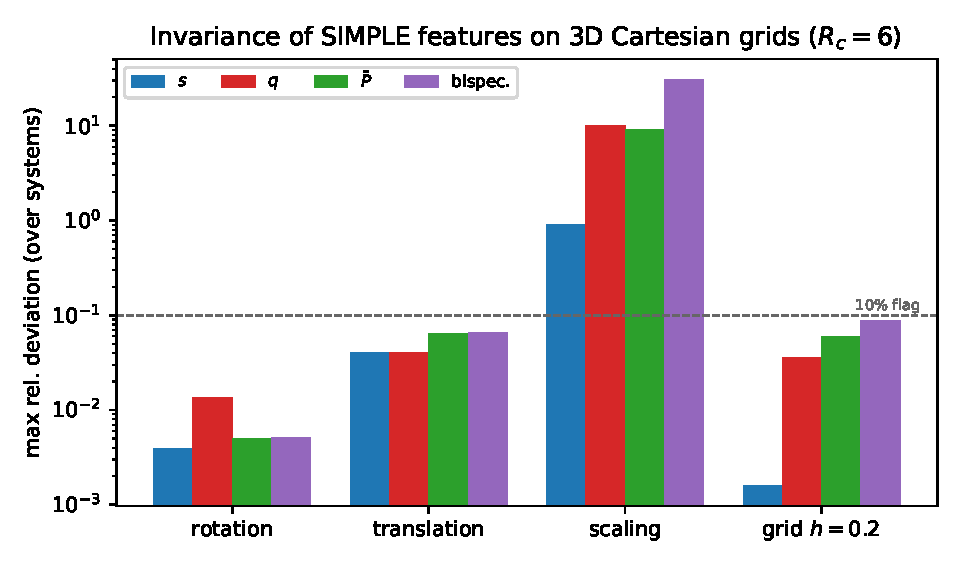
\includegraphics[width=\columnwidth]{figures/invariance_summary.pdf}
\caption{SIMPLE invariants at the fixed production settings ($\Rc=6$~bohr, $\nout=10$,
$\nin=20$; $\Lambda_{\max}=\nin/\nout=2$), pooled over the five test systems (box:
quartiles; whiskers: 5--95\%; points: outliers; dashed line: the $10\%$ flag).
\textbf{(a)} \emph{Invariance} --- relative deviation of each family ($s$, $q$, power
spectrum $\tilde P$, bispectrum) under random rotation, sub-grid translation, uniform
scaling (within $\lambda\le\Lambda_{\max}$), and grid refinement vs the continuum.
Rotation, translation, and grid refinement are well controlled; under scaling the power
spectrum and bispectrum stay near $1\%$ and the reduced gradient near $10\%$ (it is the
most resolution-demanding and tightens with $\nin$; App.~\ref{app:stress}).
\textbf{(b)} \emph{Reconstruction accuracy} --- relative error of the reconstructed $s$
and $q$ against the exact (finite-difference) gradient/Laplacian: $s$ is accurate
($\sim$few percent), whereas $q$ is wrong by factors up to $\sim$$10^2$ in dense
environments. The reduced gradient and the spectra are thus both invariant and accurate,
while the reduced Laplacian is not reconstructable and is excluded. Detailed per-test
panels are in App.~\ref{app:stress}.}
\label{fig:cartesian}
\end{figure}

\subsection{Exchange-hole functional}
\label{sec:results-hole}

Being spherically symmetric, the functional uses only the $N_C$ monopole channels
(plus the fixed $\ell=1$ gradient operator for the second-order term), so a
self-consistent step costs $2N_C$ convolutions --- the forward descriptors
$\{C_n\}$ and the adjoint potential [Eq.~\eqref{eq:adjoint}] --- with $N_C=24$ here.
The production functional is the second-order GEA hole, a single deformation constant
($R=-0.12$, equivalently $A_{s^2}=-1.01$) --- the one-time homogeneous-gas envelope
response of Eq.~\eqref{eq:amp}, not fit to any atomic data --- on a single cutoff
$\Rc=3$~\AA, run self-consistently (Sec.~\ref{sec:impl}).

On the closed-shell set it improves the bare hole toward exact exchange for every
atom and is near-exact for the lightest (Table~\ref{tab:energies}): He $-1.0019$
(exact; the Fermi--Amaldi limit), Be $-1.927$ ($+0.006$ vs OEP), Ne $-5.461$
($+0.060$ vs HF) --- competitive with or better than PBE (Be $+0.035$, Ne $+0.102$)
and comparable to rSCAN. The dense atom Mg over-binds ($+0.28$), the finite-window
limitation of a single-cutoff hole. With the gauge fix of Sec.~\ref{sec:impl} the He
HOMO eigenvalue is $-0.910$~Ha against the OEP $-0.913$~Ha, giving the correct
Koopmans ionization potential. Figure~\ref{fig:vx} compares the self-consistent
SIMPLE exchange potential to the optimized effective
potential~\cite{Talman_1976,Krieger_1992} for He, Be, Ne; the potentials agree
through core and valence and reproduce the $-1/r$ tail. Open-shell atoms (N, P)
require the unrestricted exact-exchange reference (Sec.~\ref{sec:hole}) and are
deferred to the full benchmark.

\begin{figure}[tb]
\centering
\PH{figures/simple\_hole\_vx.pdf — regenerated in Phase D}
\caption{Self-consistent SIMPLE exchange potential versus OEP for \PH{three
atoms}.}
\label{fig:vx}
\end{figure}

\begin{table}[tb]
\centering
\caption{Exchange-only energies (Ha) for closed-shell atoms: the second-order GEA
SIMPLE hole (this work) and the bare hole versus exact exchange (OEP; HF for Ne, Ar
where OEP is unavailable/unreliable), with PBE~\cite{Perdew_1996} and
rSCAN~\cite{Bart_k_2019} for reference. The GEA hole improves the bare hole toward
exact exchange for every atom and is near-exact for the lightest; Mg over-binds, the
single-cutoff finite-window limitation. (Spin treatment per Sec.~\ref{sec:hole};
open-shell N, P require the unrestricted reference and are deferred.)}
\label{tab:energies}
\begin{tabular}{lccccc}
\toprule
Atom & exact-x & bare & GEA hole & PBE & rSCAN \\
\midrule
He & $-1.0019$ & $-1.0019$ & $-1.0019$ & $-0.9705$ & $-0.9971$ \\
Be & $-1.9208$ & $-1.9867$ & $-1.9268$ & $-1.8853$ & $-1.9105$ \\
Ne & $-5.4012$ & $-5.5787$ & $-5.4607$ & $-5.2989$ & $-5.4110$ \\
Mg & $-6.8577$ & $-7.2064$ & $-7.1407$ & $-6.7599$ & $-6.8878$ \\
Ar & --- & $-5.4047$ & $-5.2756$ & $-5.0318$ & $-5.4515$ \\
\bottomrule
\end{tabular}
\PH{Regenerate via the full benchmark driver (KS gaps; open-shell N/P vs unrestricted
$E_x^U$); rSCAN where it converges.}
\end{table}

\bibliography{refs}

% =====================================================================
\appendix
% Pedagogical appendix: all derivations, followable by a first-year
% engineering graduate student. Included from main.tex after \appendix.

\section{The orthonormal local expansion}
\label{app:basis}

We expand the density inside a ball $B_{\Rc}$ in a product basis of real spherical
harmonics and radial functions. The radial functions are spherical Bessel
functions truncated to the ball with Dirichlet (vanishing) boundary conditions,
\begin{equation}
R_{n\ell}(r)=\mathcal N_{n\ell}\,j_\ell\!\left(\frac{z_{n\ell}\,r}{\Rc}\right),
\qquad j_\ell\!\left(z_{n\ell}\right)=0,
\end{equation}
where $z_{n\ell}$ is the $(n{+}1)$th positive zero of $j_\ell$. The constants
$\mathcal N_{n\ell}$ are fixed by orthonormality with the radial measure $r^2dr$,
$\int_0^{\Rc} r^2 R_{n\ell}R_{n'\ell}\,dr=\delta_{nn'}$, which follows from the
Sturm--Liouville orthogonality of the Bessel functions. Why this basis? The
$j_\ell$ are eigenfunctions of the radial Laplacian,
$\nabla^2[j_\ell(kr)\Ylm]=-k^2 j_\ell(kr)\Ylm$, so derivatives act diagonally
(used in App.~\ref{app:gea}); and the Dirichlet truncation makes the set complete
and orthonormal on the finite ball, which is what lets integrals collapse to sums
(App.~\ref{app:operators}).

The coefficients $c_{n\ell m}(\rr_0)=\int_{B_{\Rc}}K_{n\ell m}(\rr)
\rho_\sigma(\rr_0+\rr)\,d^3r$ are an exact, invertible representation of the local
density up to the truncation $n<\nin$, $\ell\le\ell_{\max}$: by orthonormality
$\rho_\sigma(\rr_0+\rr)=\sum_{n\ell m}c_{n\ell m}(\rr_0)K_{n\ell m}(\rr)$ inside
the ball. Each coefficient is a convolution of the density with a fixed kernel,
hence a single fixed stencil per channel on a grid.

A useful identity, used repeatedly, is the monopole integral of a basis function,
\begin{equation}
\label{eq:An}
A_n(R)=\int_{B_R}K_{n00}\,d^3r=\sqrt{4\pi}\int_0^R r^2 R_{n0}(r)\,dr,
\end{equation}
which for the Dirichlet basis evaluates in closed form and gives the constant-density
projection $c_{n00}=\rho\,A_n(R)$, with the ratio $A_n/A_0=(-1)^n/(n+1)$ used below.

\section{The scale transform}
\label{app:scale}

This appendix derives the scale-invariance construct of Sec.~\ref{sec:scale}.

\paragraph*{The problem.}
We want features that do not change when the density is uniformly scaled,
$\rho_\lambda(\rr)=\lambda^3\rho(\lambda\rr)$ (this normalization keeps the
electron count fixed). Exact scale invariance is obtained by choosing the cutoff
to follow the local Fermi wavelength, $\Rc\propto\bar\kF^{-1}$; but a
density-dependent cutoff cannot be implemented as a single fixed convolution
stencil. SIMPLE keeps a fixed physical window and \emph{reconstructs} the
adaptive-window descriptors by a linear map.

\paragraph*{The dilation identity [Eq.~\eqref{eq:dilation}].}
Substitute $\rr\to\rr/\lambda$ in the projection Eq.~\eqref{eq:projection} and
evaluate the coefficients of the scaled density at the scaled cutoff $R/\lambda$.
Because each basis function depends on $r$ only through the dimensionless ratio
$z_{n\ell}r/R$, the integrand keeps its shape and only prefactors survive: the
$\lambda^3$ from $\rho_\lambda$, a $\lambda^{-3}$ from $d^3r$, and a
$\lambda^{-3/2}$ from the normalization $\mathcal N_{n\ell}\propto R^{-3/2}$
combine to the $\lambda^{3/2}$ of Eq.~\eqref{eq:dilation}. At $\ell=0$ this says
the fixed-window coefficients are samples of the spherical Bessel transform of the
unscaled density at \emph{dilated} wavevectors: scaling moves the sampling points
but loses no information, provided the window still contains the density.

\paragraph*{Why subtract the window mean [Eqs.~\eqref{eq:meansplit}--\eqref{eq:transfer}].}
The Dirichlet basis vanishes at $\Rc$, but a generic density does not, so directly
re-projecting carries slowly-decaying boundary oscillations (for the HEG, where
the density is pure boundary mismatch, this is a $10\%$ effect). Transferring the
fluctuation about the window average and adding back the mean analytically through
the monopole integrals $A_n$ [Eq.~\eqref{eq:An}] removes the effect: for a uniform
density the fluctuation $\tilde c\equiv0$, so the transfer is exact at any
truncation --- this is why the HEG limit is exact by construction
(Fig.~\ref{fig:heg}).

\begin{figure}[tb]
\centering
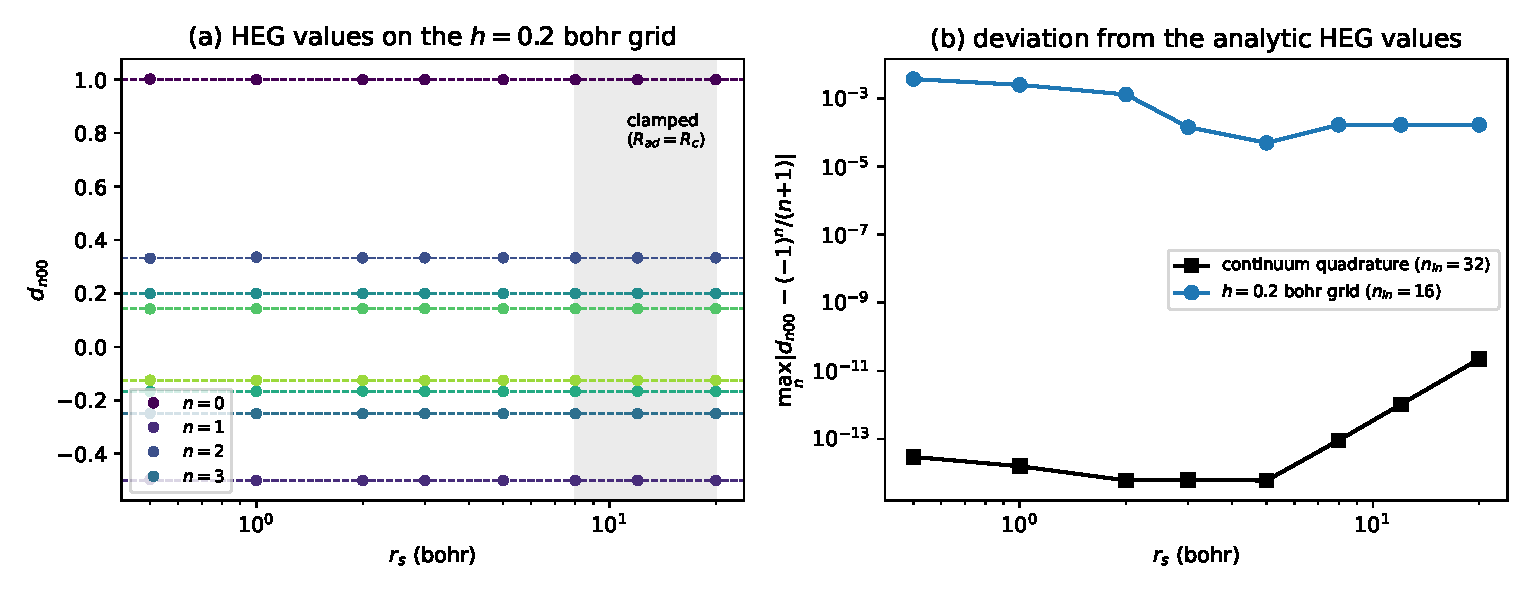
\includegraphics[width=\columnwidth]{figures/simple_heg.pdf}
\caption{Numerical verification of the homogeneous-electron-gas (HEG) limit through
the full SIMPLE pipeline (window projection, adaptive radius, mean-split transfer,
non-dimensionalization), referenced from Sec.~\ref{sec:results-features}.
\textbf{(a)} The monopole descriptors $d_{n00}$ on the $h=0.2$~bohr grid (points)
against the analytic HEG values $d^{\mathrm{HEG}}_{n00}=(-1)^n/(n+1)$ (dashed), over
$r_s\in[0.5,20]$; the shaded region marks densities where the adaptive radius is
clamped ($\Rad=\Rc$), which leaves the HEG values unaffected. \textbf{(b)} Maximum
deviation from the analytic values versus $r_s$: the continuum pipeline reproduces
them to ${\sim}2\times10^{-11}$ (exact by construction; residual from the root-find
tolerance), and the $h=0.2$~bohr grid to $<4\times10^{-3}$ (kernel-quadrature error).}
\label{fig:heg}
\end{figure}

\paragraph*{The closed form [Eq.~\eqref{eq:transfer-closed}].}
The transfer matrix is the radial overlap of an adaptive-window basis function
with a fixed-window one. For two solutions $j_\ell(ar),j_\ell(br)$ of the
spherical Bessel equation ($a=z_{m\ell}/\Rad$, $b=z_{n\ell}/\Rc$) the
Sturm--Liouville cross-product identity integrates the overlap in closed form,
Eq.~\eqref{eq:transfer-closed}, with no quadrature or tabulation. At $R=\Rad$ the
first bracket term vanishes because $j_\ell(a\Rad)=j_\ell(z_{m\ell})=0$.
(Tabulating in the ratio $\Rad/\Rc$ fails: the high-$n$ elements oscillate on the
scale $\pi/z_{n\ell}$, so naive interpolation is inaccurate --- the closed form is
load-bearing.) Near-degenerate pairs $a\approx b$ use the analytic limit of
Eq.~\eqref{eq:transfer-closed}; when $\Rad=\Rc$ (clamped) the transfer is the
identity. Crucially $\mathsf M^{(\ell)}$ acts only on the radial index $n$,
identically for every $m$ --- the property that makes the transform commute with
rotations (App.~\ref{app:nondim}).

\section{Non-dimensionalization and invariance}
\label{app:nondim}

The descriptors are normalized at the adaptive radius,
$d_{n\ell m}=c'_{n\ell m}/[A_0(\Rad)\bar\rho_{\sigma,\mathrm{safe}}(\Rad)]$. Under
scaling, $A_0(\Rad/\lambda)=\lambda^{-3/2}A_0(\Rad)$ and
$\bar\rho_\sigma\mapsto\lambda^3\bar\rho_\sigma$, so the denominator scales as
$\lambda^{3/2}$, exactly cancelling the $\lambda^{3/2}$ of the numerator from
Eq.~\eqref{eq:dilation}: $d_{n\ell m}$ is invariant for every $\ell$, up to
$\rho_{\min}$ effects and the transfer truncation. (This corrects an earlier
convention that multiplied by $\bar\kF^\ell$, which actually multiplies the
fixed-$\xi$ features by $\lambda^\ell$ and breaks the invariance it was meant to
support; an order-unity balance across $\ell$ may instead be restored by a
\emph{constant} $(\xi^*)^{-\ell}$, which affects neither covariance nor
invariance.)

\paragraph*{Rotational covariance.}
Under a rotation $\mathcal R$, the raw coefficients transform as rank-$\ell$
tensors, $c_{n\ell m}\mapsto\sum_{m'}D^{(\ell)}_{mm'}(\mathcal R)c_{n\ell m'}$.
The transform preserves this because (i) $\Rad$ depends only on the invariant ball
average; (ii) $\mathsf M^{(\ell)}$ acts on $n$, not $m$; (iii) the mean split
touches only the invariant $(0,0)$ channel. Since the transfer acts on the radial
slot and the rotation on the magnetic slot, they commute,
\begin{equation}
\label{eq:commute}
\bigl(\mathsf M^{(\ell)}\otimes\mathbb 1\bigr)\bigl(\mathbb 1\otimes D^{(\ell)}\bigr)
=\bigl(\mathbb 1\otimes D^{(\ell)}\bigr)\bigl(\mathsf M^{(\ell)}\otimes\mathbb 1\bigr),
\end{equation}
so $d_{n\ell m}$ is a rank-$\ell$ tensor and any contraction to total angular
momentum zero is invariant (verified numerically to $\lesssim2\times10^{-15}$).

\paragraph*{Low-density limit.}
With the safe floor $\bar\rho_{\sigma,\mathrm{safe}}=(\bar\rho_\sigma^2+\rho_{\min}^2)^{1/2}$,
as $\rho\to\epsilon\rho$ the adaptive radius clamps at the window and the descriptors
reduce to fixed-window coefficients divided by a floor: $d_{n\ell m}=\mathcal O(\epsilon)$
and $\tilde P_{n\ell}=\sum_m d_{n\ell m}^2=\mathcal O(\epsilon^2)$, smoothly and
without overflow, with crossover at $\epsilon^*=\rho_{\min}/\bar\rho_\sigma$.

\begin{figure}[tb]
\centering
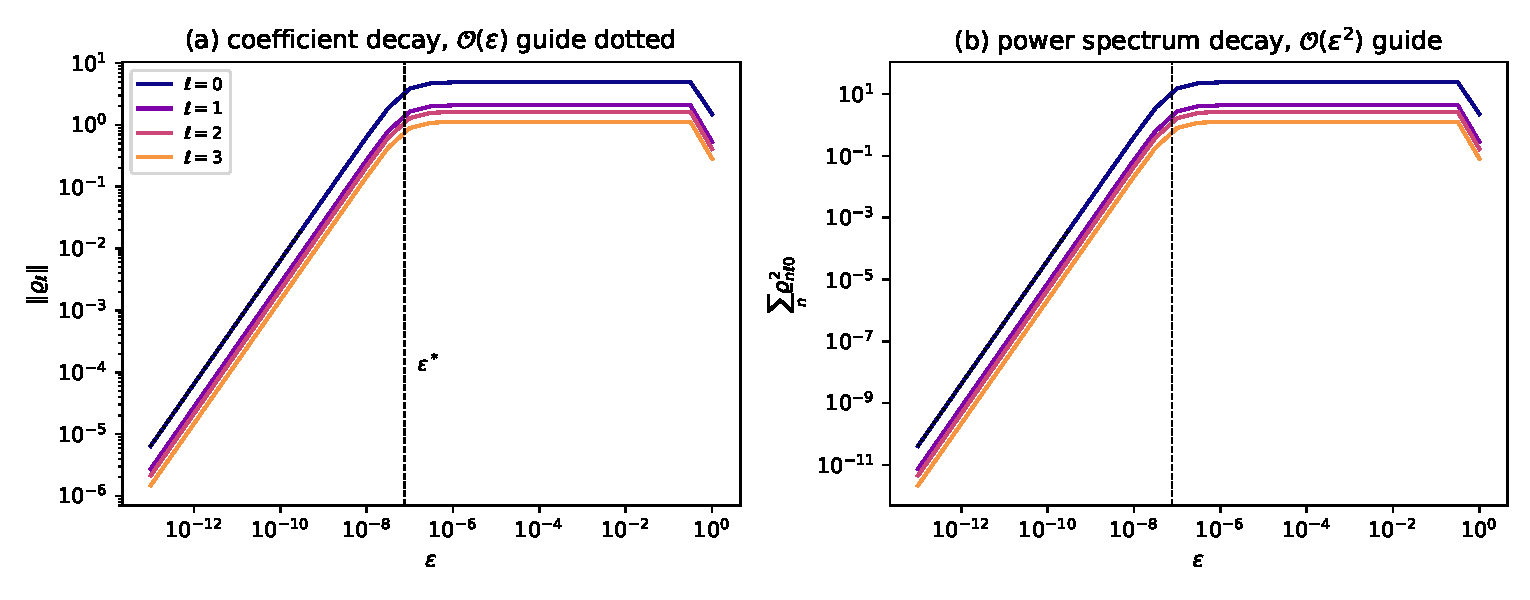
\includegraphics[width=\columnwidth]{figures/simple_vacuum.pdf}
\caption{Low-density (vacuum) stability of the descriptors as the density is scaled
down uniformly, $\rho\mapsto\epsilon\rho$, over thirteen decades of $\epsilon$. The
descriptor-coefficient norm $\lVert d_{n\ell m}\rVert$ (blue) decays as
$\mathcal O(\epsilon)$ and the power spectrum $\tilde P_{n\ell}=\sum_m d_{n\ell m}^2$
(orange) as $\mathcal O(\epsilon^2)$ (reference slopes shown dashed; the fitted
power-spectrum slope is $2.000$), exactly as predicted in this section: below the
crossover $\epsilon^*=\rho_{\min}/\bar\rho_\sigma$ the safe floor
$\bar\rho_{\sigma,\mathrm{safe}}$ takes over and the descriptors vanish smoothly and
without overflow rather than diverging by division by a vanishing mean density. This
is the property that lets the functional be evaluated in near-vacuum tail regions of
real atoms.}
\label{fig:vacuum}
\end{figure}

\section{Operator projections}
\label{app:operators}

\paragraph*{Multilinear functionals as sums.}
Any $\nu$-point integral functional with a rotation-invariant kernel,
$\mathcal O_\nu[\rho](\rr_0)=\int_{B_{\Rc}}\!\cdots\!\int\mathcal K_\nu(\rr_1,\dots,\rr_\nu)
\prod_i\rho(\rr_0+\rr_i)\,d^3r_i$, becomes, on inserting the expansion
$\rho(\rr_0+\rr)=\sum c_{n\ell m}K_{n\ell m}(\rr)$,
\begin{equation}
\begin{aligned}
\mathcal O_\nu[\rho]&=\sum_{\{n_i\ell_i m_i\}}T^{(\nu)}_{\{n_i\ell_i m_i\}}\prod_{i=1}^\nu c_{n_i\ell_i m_i},\\
T^{(\nu)}&=\int\!\cdots\!\int\mathcal K_\nu\prod_i K_{n_i\ell_i m_i}\,d^3r_i .
\end{aligned}
\end{equation}
The projected-kernel tensor $T^{(\nu)}$ is computed once. Rotation invariance of
$\mathcal K_\nu$ forces the magnetic indices to couple to total angular momentum
zero, which is exactly Clebsch--Gordan coupling; the power spectrum ($\nu=2$),
bispectrum ($\nu=3$), and higher CG trees therefore form a complete basis for
rotationally invariant multilinear functionals. Non-dimensionalization only
rescales $T^{(\nu)}$ by scalar prefactors and does not change the admissible class.

\paragraph*{The Coulomb operator is a monopole.}
For the exchange-relevant kernel $\mathcal K=1/u$ acting on the density at
displacement $\uu$, the angular integral $\oint d\Omega_u\,(1/u)\,
\rho(\rr_0+\uu)$ projects out only the $\ell=0$ component, because $1/u$ is
isotropic and the higher harmonics integrate to zero. Hence the projected Coulomb
operator acts through the monopole descriptors alone,
\begin{equation}
\bar\rho(r_0,u)=\frac{1}{4\pi}\oint\rho(r_0+\uu)\,d\Omega_u=\sum_n C_n(r_0)R_n(u) ,
\end{equation}
with monopole descriptors $C_n=(P_n\rho)(r_0)$, where $\{P_n\}$ are fixed window
operators. The Coulomb operator acting on this monopole density is then a weighted
sum over the descriptors [Eq.~\eqref{eq:coulomb}],
\begin{equation}
\begin{aligned}
\int_{B_{\Rc}}\!\frac{\rho(r_0+\uu)}{u}\,d^3u
&=4\pi\!\int_0^{\Rc}\!\bar\rho(r_0,u)\,u\,du\\
&=\sum_n w_n C_n(r_0),
\end{aligned}
\end{equation}
with $w_n=4\pi\int_0^{\Rc}R_n(u)\,u\,du$. The $1/u$ weight reduces the radial
measure from $u^2du$ to $u\,du$: this is how the long-range $1/r$ structure that
semilocal functionals miss enters, and it is the foundation of the exchange-hole
functional below.

\section{Reduced gradient and Laplacian from the expansion}
\label{app:gea}

The gradient expansion of exchange,
$E_x=\int\varepsilon_x^{\mathrm{LDA}}(\rho)\bigl[1+\mu s^2+\dots\bigr]\rho\,d^3r$,
requires the reduced gradient $s=|\nabla\rho|/(2\kF\rho)$ and reduced Laplacian
$q=\nabla^2\rho/(4\kF^2\rho)$, with $\kF=(3\pi^2\rho)^{1/3}$. We extract both from
the SIMPLE expansion with parameter-free spectral operators.

\paragraph*{Gradient (slope at origin).}
The density at the expansion center along a ray is built from the $\ell=1$
channel; its slope at $r_0$ is $\rho'(r_0)=\sum_n a^{(1)}_n R'_{n1}(0)$, where
$a^{(\ell)}_n$ are the channel-$\ell$ radial expansion coefficients and
$R'_{n1}(0)=\mathcal N_{n1}k_n/3$ (the small-argument behavior $j_1(x)\approx x/3$).
This is a fixed linear operator on the gridded density.

\paragraph*{Laplacian (Bessel eigenvalue).}
Because $\nabla^2[R_{n0}]=-k_n^2 R_{n0}$ with $k_n=z_{n0}/\Rc$, the Laplacian is the
eigenvalue-weighted monopole sum $\nabla^2\rho(r_0)=-\sum_n a^{(0)}_n k_n^2 R_{n0}(0)$.
This must be evaluated \emph{per channel}: the coefficients
$a^{(0)}_n=\int_0^{\Rc} R_{n0}(u)\,\rho_0(u;r_0)\,u^2\,du$ are formed first --- they
decay for a smooth density --- and the growing $k_n^2$ weights applied afterward, so
the sum converges. Folding the weights into a single kernel
$\sum_n(-k_n^2 R_{n0}(0))R_{n0}(u)$ \emph{before} the density integral builds a
near-singular ($\sim\nabla^2\delta$) object whose huge oscillatory values destroy the
result to catastrophic cancellation; the $k_n^2$ growth makes this fatal for $\ell=0$
(the $\ell=1$ gradient, growing only as $k_n^1$, is stable either way). The operator
is therefore matrix-free and applied per channel.

\paragraph*{Constant annihilation and the uniform limit.}
The $\ell=1$ gradient operator ends with
$\mathsf O\to\mathsf O-\mathrm{diag}(\sum_j\mathsf O_{ij})$, forcing
$\mathsf O[\text{const}]=0$ (the gradient of a uniform density vanishes; the
subtraction also removes the DC truncation residual). The $\ell=0$ Laplacian is
\emph{not} constant-annihilated: for the $k_n^2$ channel the constant's own
truncation residual is large (a constant does not decay in the window), so
subtracting it would contaminate every point. The operator is instead applied to
densities that decay within the window (real pseudopotential atoms), where
$\nabla^2\rho$ is recovered directly to $\sim1\%$ in the core/valence (verified
against finite differences); the uniform-density limit $q\to0$ is imposed
analytically in the functional, not through this operator.

\paragraph*{In SIMPLE features.}
Dividing these dimensional operators by the non-dimensionalization amplitude turns
them into the feature contractions of Eq.~\eqref{eq:sq}: the spectral weights are
$g^{(1)}_n\propto R'_{n1}(0)$ (slope-at-origin) acting on the $\ell=1$ features
$d_{n1m}$, and $g^{(0)}_n\propto k_n^2 R_{n0}(0)$ (Bessel eigenvalue) acting on the
$\ell=0$ features $d_{n00}$. The reduced gradient is the norm of the $\ell=1$
contraction --- hence the $\ell=1$ power of the spectrally-weighted features --- and
the reduced Laplacian is the $\ell=0$ contraction.

\paragraph*{The $10/81$ coefficient.}
For the ball-normalized reduced gradient the second-order gradient-expansion
coefficient comes out to the standard $\mu=10/81$~\cite{Antoniewicz_1985} on the
single-scale path that atoms occupy, with $\kappa=s_{\mathrm{SIMPLE}}/s_{\mathrm{phys}}\to1$
in the high-density limit --- derived, not fit. Extracting derivatives from a
finite truncated expansion has intrinsic limits: the spectral operators require a
smooth density (a bare nuclear cusp breaks them, but pseudopotential densities are
smooth) and the full window with $\sim40$ channels; the far tail degrades where
the finite-difference reference is itself noisy.

\section{The exchange-hole functional: full derivation}
\label{app:hole}

We reconstruct the functional from the exact hole, flagging each degree of freedom
(DOF) that is dropped or constrained, so the model's location relative to the exact
functional is explicit.

\paragraph*{Exact starting point.}
The exchange energy is exactly Eq.~\eqref{eq:exact-hole} with
$n_x(r_0,\uu)=-|\rho_1(r_0,r_0+\uu)|^2/\rho(r_0)$, $\rho_1$ the one-particle
density matrix. The hole obeys the sum rule $\int d^3u\,n_x=-1$, the on-top value
$n_x(r_0,\mathbf 0)=-\tfrac12\rho(r_0)$, and $n_x\le0$. The full object is a
two-point function with arbitrary angular dependence in $\uu$.

\paragraph*{DOF \#1 --- convolutional ansatz.}
We factor the hole into the actual neighboring density, a single universal shape
$S$, and two local scalars:
$n_x(r_0,\uu)=-\rho(r_0+\uu)S(\zeta(r_0)u)/\mathcal N(r_0)$. The neighboring-density
factor retains genuine non-local information; the \emph{shape} is collapsed to one
function plus a local inverse-length scale $\zeta$ and a normalization $\mathcal N$.

\paragraph*{DOF \#2 --- monopole projection (decisive).}
Inserting the ansatz into Eq.~\eqref{eq:exact-hole}, the $1/u$ weight selects the
spherical average of $\rho(r_0+\uu)$, so only the $\ell=0$ multipole survives
(App.~\ref{app:operators}): $\bar\rho(r_0,u)=\sum_n C_n(r_0)R_n(u)$. The model is
intrinsically a spherically symmetric hole; \emph{every $\ell\ge1$ hole multipole
is dropped here.} This is the largest DOF loss and is the source of the residual
open-shell error.

\paragraph*{Closed kernel (no DOF lost).}
With $S$ fixed, the $u$-integrals precompute into the envelope tables
$\alpha_n(\zeta)=\int_0^\infty S(\zeta u)R_n(u)u^2du$ and
$\beta_n(\zeta)=\int_0^\infty S(\zeta u)R_n(u)u\,du$. The number enclosed and the
self-Coulomb of the enclosed density are linear contractions
$Q_S(\zeta)=\bm\alpha(\zeta)\!\cdot\!\mathbf C$ and
$\Phi_S(\zeta)=\bm\beta(\zeta)\!\cdot\!\mathbf C$,
giving the boxed self-energy $\varepsilon_x=-\tfrac12\Phi_S/Q_S$
[Eq.~\eqref{eq:eps-x}]: exchange per electron is $-\tfrac12$ the self-Coulomb of
the enclosed density divided by the number enclosed.

\paragraph*{DOF \#3 --- closing the scale, and the exact limits.}
One scalar per point remains, fixed by the on-top sum rule $Q_S(\zeta)=2$ (a
spin-paired pair). This is where the limits enter:
\begin{itemize}
\item \emph{HEG/LDA.} Uniform $\rho\Rightarrow\bar\rho$ constant; with the HEG hole
$S(x)=[3j_1(x)/x]^2=[j_0(x)+j_2(x)]^2$, $Q_S=2\Rightarrow \zeta=\kF$ and
$\varepsilon_x\to\varepsilon_x^{\mathrm{LDA}}$. Exact by construction; here $S$ is
frozen to the HEG shape.
\item \emph{Fermi--Amaldi.} Low density / one electron $\Rightarrow Q_S<2$,
giving the self-interaction-corrected form with the full enclosed density --- exact
for H/He.
\end{itemize}
The ``2'' is a spin assumption (a paired pair); the open-shell case is handled by
the spin decomposition of App.~\ref{app:spin}.

\paragraph*{Recovering the gradient expansion.}
Inhomogeneity is returned to the shape by adding $\ell\ge1$ Bessel modes that
vanish at the origin (preserving on-top and HEG),
$S(x;\{c\})=[\,j_0(x)+j_2(x)+\sum_m c_m\varphi_m(x)]^2$ with
$\varphi_m=j_\ell(\kappa_m x)$ (mode wavevectors $\kappa_m$) and deformation
coefficients $c_m=\sum_\alpha A^m_\alpha I_\alpha[\rho]$ (coefficients $A^m_\alpha$)
linear in the SIMPLE invariants $I_\alpha$. The invariants vanish for a uniform density
(preserving LDA), and the small-$s$ slope of $c_m$ is fixed by the gradient
expansion ($\mu=10/81$ at second order, optionally fourth order). The bare
parameter-free functional uses only the monopole and gradient features and so is
spherically symmetric.

\paragraph*{Calibrating the deformation (one-time HEG response).}
The map from the invariants to the envelope amplitude is fixed, not fit. To linear
order the envelope deformation shifts the enhancement factor by
$\delta F_x=\sum_m\rho_m\,c_m$, where the \emph{envelope response}
$\rho_m\equiv\partial F_x/\partial c_m$ is evaluated once at the homogeneous gas:
perturb the amplitude $c_m$ about the bare hole ($c=0$), re-solve the on-top scale
$Q_S(\zeta)=2$, and read off the change in $F_x=\varepsilon_x/\varepsilon_x^{\mathrm{unif}}$.
The coefficients are then chosen so $\sum_m\rho_m A^m_\alpha$ equals the
gradient-expansion coefficient of invariant $\alpha$ [the $10/81$, $146/2025$,
$-73/405$ of Eq.~\eqref{eq:fx}]; with a single mode this is simply
$A_\alpha=(\text{coefficient}_\alpha)/\rho_0$. Because $F_x$ and the invariants are
scale-free, $\rho_0$ is universal (computed once), so the deformed functional
reproduces Eq.~\eqref{eq:fx} by construction while the bare-hole limits survive.

\paragraph*{The DOF ledger and the frontier.}
\begin{center}
\renewcommand{\arraystretch}{1.2}
\begin{tabular}{p{0.40\columnwidth}p{0.30\columnwidth}p{0.16\columnwidth}}
\toprule
DOF dropped/constrained & where & restored? \\
\midrule
arbitrary radial profile $\to$ one $S(\zeta u)$ & convolution ansatz & partly \\
all $\ell\ge1$ hole multipoles & monopole projection & \textbf{no} \\
envelope shape frozen to HEG & $Q_S=2$ closure & by deformation \\
local scale $\zeta$ + spin (paired) & on-top rule & no \\
\bottomrule
\end{tabular}
\end{center}
The unremoved residual --- a $\sim10\%$ over-binding on strongly open,
partially-filled subshells --- is DOF \#2: that exchange is carried by the
$\ell\ge1$ hole multipoles, and no deformation of a spherically symmetric envelope
can supply them. The natural extension is an explicit multipole hole
$n_x(r_0,\uu)=\sum_\ell n_x^{(\ell)}(r_0,u)P_\ell(\rhat\!\cdot\!\hat r_0)$ using the
$\ell\ge1$ SIMPLE projections as genuine hole channels.

\section{Spin conventions}
\label{app:spin}

Exchange acts within each spin channel, so the spin-resolved energy follows from
the spin-scaling relation
$E_x[\rho_\uparrow,\rho_\downarrow]=\tfrac12\bigl(E_x[2\rho_\uparrow]+E_x[2\rho_\downarrow]\bigr)$.
For a spin-paired system $\rho_\uparrow=\rho_\downarrow=\rho/2$, this reduces to the
total-density expressions used in the main text, with the on-top count of $2$. For
open shells we evaluate the spin-restricted functional on $2\rho_\sigma$ in each
channel and combine; the Hartree--Fock/OEP reference used for comparison is itself
spin-restricted, which under-counts open shells, so the unrestricted-exact
correction is applied when comparing.

\section{Self-consistent potential and numerical details}
\label{app:hole-numerics}

\paragraph*{Convolutional adjoint potential.}
Each monopole descriptor is a convolution of the density with a fixed kernel,
\begin{equation}
\label{eq:descriptor-conv}
C_n(\rr)=\int K_n(\rr'-\rr)\,\rho(\rr')\,d^3r'=(K_n*\rho)(\rr),
\end{equation}
so that $\delta C_n(\rr')/\delta\rho(\rr)=K_n(\rr-\rr')$. With the exchange energy
$E_x=\int\rho\,\varepsilon_x[\{C_n\}]\,d^3r$, the potential is the explicit
variational derivative, following Ref.~\cite{Sahoo2024},
\begin{equation}
\label{eq:adjoint}
\begin{aligned}
v_x(\rr)&=\frac{\delta E_x}{\delta\rho(\rr)}\\
&=\varepsilon_x(\rr)+\sum_n\int d^3r'\,\rho(\rr')\,
\frac{\partial\varepsilon_x(\rr')}{\partial C_n}\,K_n(\rr-\rr') .
\end{aligned}
\end{equation}
The second term is itself a convolution over the kernel: each descriptor's
contribution is $K_n$ applied to $\rho\,\partial\varepsilon_x/\partial C_n$. In the
radial finite-element implementation this convolution is the transpose
$P_n^{\mathsf T}$ of the forward stencil $P_n$, weighted by the quadrature measure
$w=4\pi r^2 w_{\mathrm{quad}}$ ($w_{\mathrm{quad}}$ the radial quadrature weights),
\begin{equation}
\label{eq:adjoint-discrete}
v_x=\varepsilon_x+\sum_n \frac{P_n^{\mathsf T}\!\bigl[w\,\rho\,
\partial\varepsilon_x/\partial C_n\bigr]}{w} ,
\end{equation}
exact against finite differences of the energy.

\paragraph*{On-top scale by enclosed-charge inversion.}
The on-top scale is \emph{not} found by a nested self-consistent iteration. The
$S$-weighted enclosed charge
$Q_S(\zeta)=\bm\alpha(\zeta)\cdot\mathbf C=\int_0^\infty S(\zeta u)\,\bar\rho(r_0,u)\,4\pi u^2\,du$
uses the precomputed envelope table $\alpha_n(\zeta)$, so for the fixed monopole
descriptors $\mathbf C$ it is a single matrix--vector product on a $\zeta$-grid. As
$\zeta\to0$, $S\to1$ and $Q_S$ approaches the full window charge; as
$\zeta\to\infty$, $Q_S\to0$. Because $Q_S(\zeta)$ is monotonic, $Q_S(\zeta)=2$ has a
unique root recovered by one-dimensional inversion of the precomputed curve --- the
identical fixed-stencil enclosed-charge machinery that solves $g(\Rad)=\xi^*$ for
the adaptive radius (App.~\ref{app:scale}). The solve is therefore pointwise,
non-iterative, and vectorized over all grid points, adding no loop to the
Kohn--Sham cycle. (Confirmed in the implementation: the self-consistent functional
reproduces the direct-integral hole on the converged density.)

\paragraph*{Stiffness and the frozen-gradient dual loop.}
The exchange-kernel response $\delta v_x/\delta\rho$ is stiff. The reduced Laplacian
$q$ that carries the fourth-order GEA term [Eq.~\eqref{eq:fx}] enters the potential
through the $\ell=0$ spectral Laplacian, whose forward is stable when applied per
channel (App.~\ref{app:gea}) but whose adjoint re-forms the singular $k_n^2$ kernel
and is correspondingly ill-conditioned. This is handled by a frozen-gradient dual
loop: the gradient/Laplacian (GEA) correction is held fixed on the stable bare-hole
potential through the Kohn--Sham outer loop, which converges all atoms while keeping
the bare-hole stability bound. Quantitative validation of the dual loop on the
self-consistent atom set is part of the production benchmarks.

\paragraph*{The $-1/r$ tail.}
The exact exchange potential decays as $-1/r$. The model potential is made to
recover this by an energy-neutral gauge fix (subtracting the asymptotic constant)
together with a low-density damping $f=\rho^2/(\rho^2+\rho_c^2)$ ($\rho_c$ a small
damping density), which restores the $-1/r$ tail and the correct Koopmans
ionization potential without changing the energy.

\section{Three-dimensional Cartesian-grid validation}
\label{app:3d}

The entire pipeline is run on genuine 3D Cartesian lattices, with window
coefficients by direct kernel sums, ball averages by partial-cell shell sums
(linear-ramp weights normalized by their own sum, keeping the HEG limit exact),
and the adaptive radius, transfer, and non-dimensionalization as in 1D. Test
densities are pseudo-diatomics: pseudo-H$_2$ (two analytic $1s$ atoms,
$\rho=e^{-2r}/\pi$, $b=1.40$~bohr; nuclear cusps) and pseudo-N$_2$ (two nitrogen
pseudopotential valence densities from the radial DFT solver, GGA-PBE,
$b=2.074$~bohr; smooth). A quasi-exact continuum reference is built per-atom in an
aligned frame and rotated with real Wigner-$D$ matrices.

The descriptors converge as $\mathcal O(h^2)$ ($0.1$--$1.2\%$ at $h=0.2$~bohr,
$0.03$--$0.3\%$ at $h=0.1$); under 24 random rotations the per-channel deviation
from the covariant prediction stays at the static-quadrature level
($\lesssim8\times10^{-3}$) and the rotation-invariant power-spectrum spread is only
$2$--$8\times10^{-4}$; symmetry-forbidden odd-$\ell$ channels at the bond midpoint
vanish to machine precision ($\lesssim2\times10^{-16}$); and a sub-grid registration
sweep stays at $\sim\!1.0\times10^{-3}$. The lattice scale-invariance test tracks the 1D radial behavior
with the same two breakdown mechanisms. Thus $\sim0.2$~bohr grid spacings, typical
of real-space pseudopotential codes, are sufficient.

% =====================================================================

\end{document}
